\chapter{Optimizing Motion of External Cavity Grating}\label{GratingRatioAppendix}
In order to narrow the line width of the master laser and make it more tunable and stable, we have mounted a diffraction grating in a Littrow configuration. The gratings are mounted on piezoelectric actuators that can be automatically moved in unison by our control circuitry. 

However, in order for this to work, it is important to verify that the piezos can be scanned in such a way that the resonances of the external cavity track smoothly. In order to accomplish this, one must find a ratio that relates the relative rates at which each piezoelectric actuator is scanned. As explained in Section \ref{ensuringAbilityToFineTune}, the length of the cavity and the angle of the grating must change in such a way that the wavelength featured by each changes at the same rate for small displacements. 

For many configurations, this is not very tricky. However, at one point we discovered that for certain geometries, the appropriate ratio might be negative. To this end, we created the following Mathematica notebook to model the motion of the grating and help us to ensure that our electronics are capable of moving the actuators properly. 

In practice, the results of this calculation would typically be used only as a starting point. In order to really get the laser working well, the experimenter usually adjusts the ratio iteratively in order to maximize the range over which the frequency of the laser can be scanned without mode hopping. 

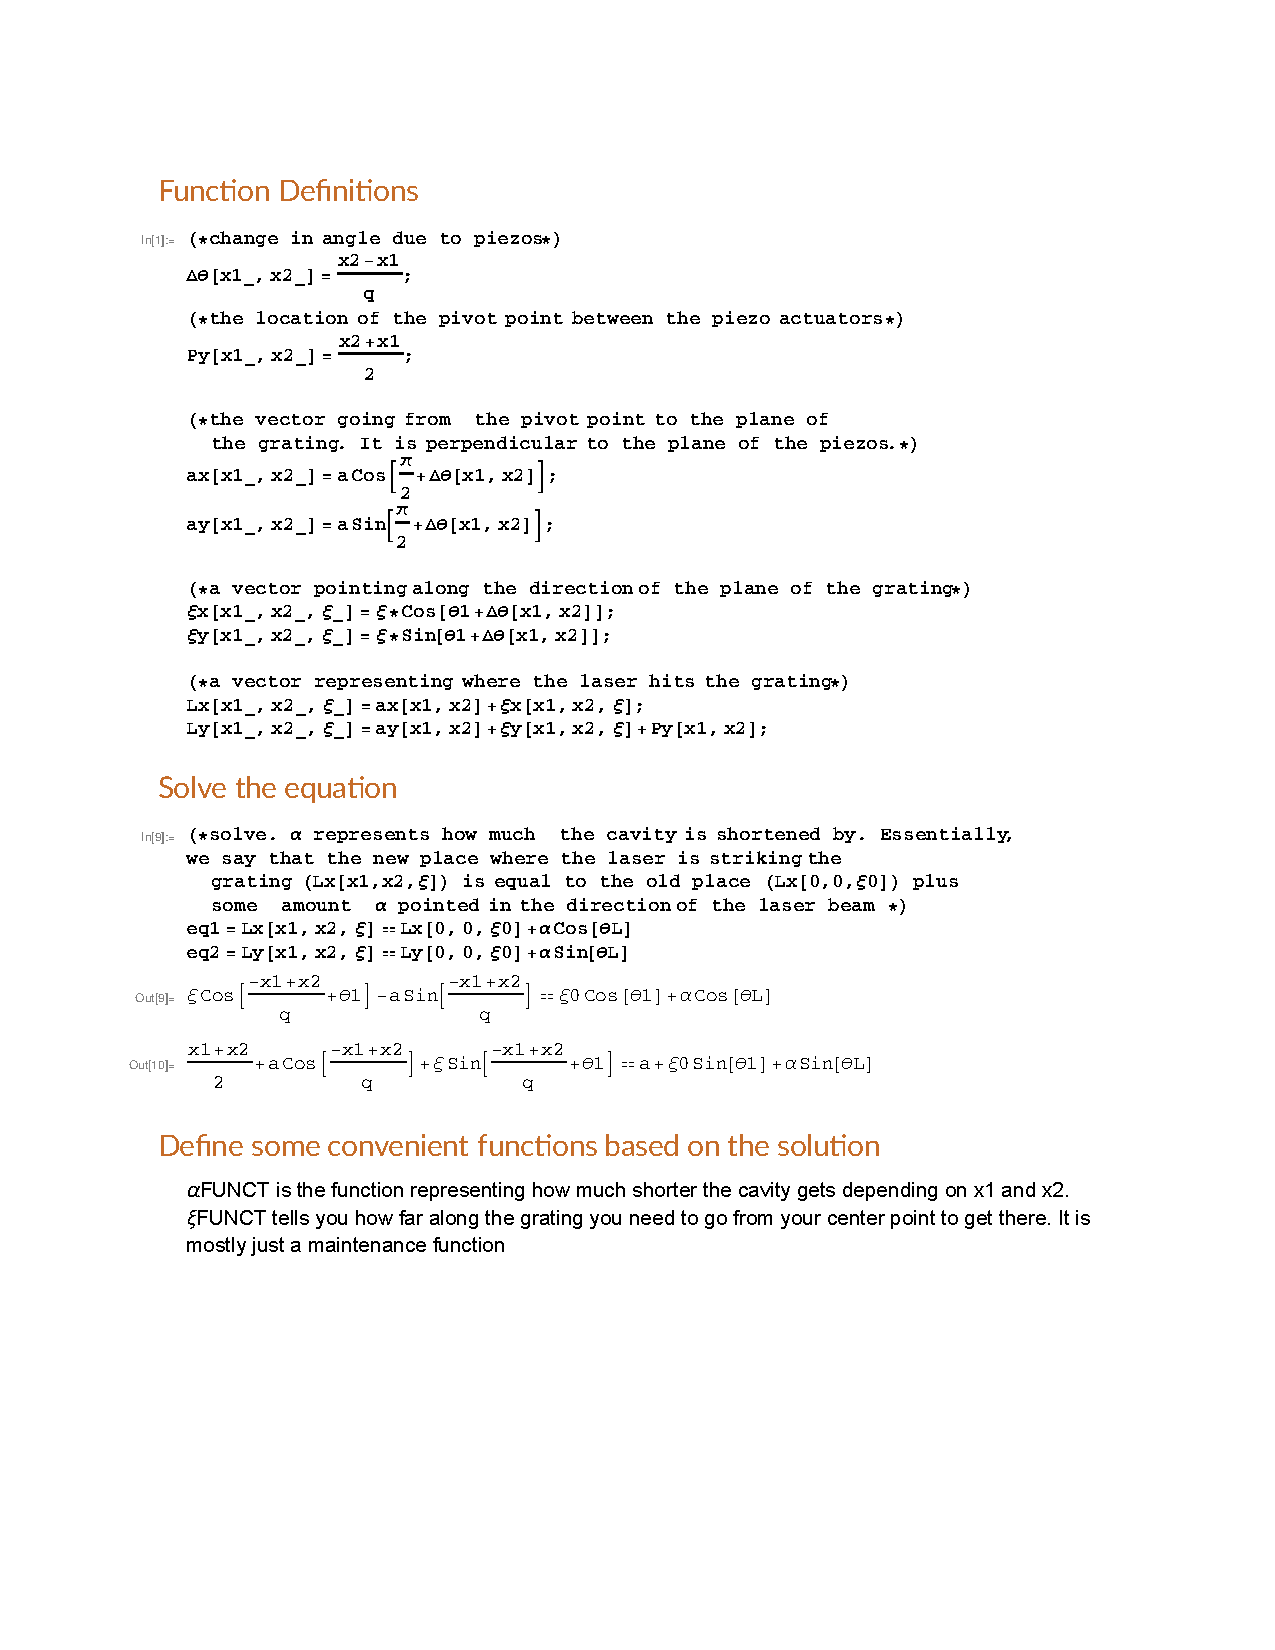
\includepdf[pages={1-10},scale=0.85]{grating_motion}


